% has to be loaded outside of a frame to work!
\maketitle

\begin{frame}[plain, noframenumbering]{Licença}
    \begin{columns}
        \begin{column}{0.5\textwidth}
            O texto e as figuras desses slides possuem uma
            \href{https://creativecommons.org/licenses/by-nc-sa/4.0/deed.pt}{Licença
            Creative Commons
            Atribuição-NãoComercial-CompartilhaIgual 4.0 Internacional (CC BY-NC-SA 4.0)}
            \vfill
            \centering
            \vspace{1em}
            
\includegraphics[width=0.2\columnwidth]{CC_NC_SA.png}
        \end{column}
        \begin{column}{0.5\textwidth}
            \centering
            
\includegraphics[width=0.8\columnwidth]{qrcode.png}
        \end{column}
    \end{columns}
    \vfill
\end{frame}

\begin{frame}{Truque da Corrente Linear\footnote{\textit{Linear Chain Trick}.} (TCL)}
	O Truque da Corrente Linear (TCL) \parencite{hurtadoGeneralizationsLinearChain2019, hurtadoProcedureDerivingNew2020, andoHowFastLinear2020}
	é usado em modelos epidemiológicos compartimentais para
	modelar tempos de espera em transições de compartimentos usando
	subcompartimentos com uma distribuição \textcolor{blue}{Erlang}\footnote{mais informações
	sobre a distribuição Erlang na \href{https://en.wikipedia.org/wiki/Erlang_distribution}{Wikipedia}.}.
	\vfill
	A distribuição Erlang é uma soma de $k$ distribuições exponenciais
	independentes.
	\vfill
	Sem subcompartimentos, a distribuição do tempo de espera se torna uma
	distribuição \textcolor{blue}{Exponencial}.
\end{frame}

\begin{frame}{Distribuição Exponencial vs Erlang}
    \begin{columns}
        \begin{column}{0.5\textwidth}
	    \begin{figure}
	    \centering
	    \begin{tikzpicture}[scale=0.5]
       	    	\begin{axis}[every axis plot, line width=2pt,
            	ylabel=FDP,
            	xlabel={$X$},
            	domain=0:5,samples=200,
            	axis x line*=bottom, % no box around the plot, only x and y axis
            	axis y line*=left, % the * suppresses the arrow tips
            	enlarge x limits=true, % extend the axes a bit
            	]

		\addplot [blue] {exponential(1)};
            	\addlegendentry{$\lambda=1$}
	    	\end{axis}
            \end{tikzpicture}
	    \caption{Distribuição Exponencial}
   	    \end{figure}
        \end{column}
        \begin{column}{0.5\textwidth}
	    \begin{figure}
            \centering
	    \begin{tikzpicture}[scale=0.5]
       	    	\begin{axis}[every axis plot, line width=2pt,
            	ylabel=FDP,
            	xlabel={$X$},
            	domain=0:5,samples=200,
            	axis x line*=bottom, % no box around the plot, only x and y axis
            	axis y line*=left, % the * suppresses the arrow tips
            	enlarge x limits=true, % extend the axes a bit
            	]

		\addplot [red] {erlang(1,1)};
            	\addlegendentry{$\lambda=1, k=1$}
		\addplot [yellow] {erlang(1,2)};
            	\addlegendentry{$\lambda=1, k=2$}
		\addplot [green] {erlang(1,3)};
            	\addlegendentry{$\lambda=1, k=3$}
	    	\end{axis}
            \end{tikzpicture}
	    \caption{Distribuição Erlang}
   	    \end{figure}
        \end{column}
    \end{columns}
    \vfill
\end{frame}

\begin{frame}{Modelos SEITD}
            \begin{figure}
                \centering
		\scalebox{0.65}{
                \begin{tikzpicture}[node distance=0.75cm,auto,>=latex',every node/.append style={align=center},int/.style={draw, circle, minimum size=0.9cm}]
			\node [int] (S) {$S$};
    			\node [int, right=of S] (E) {$E$};
    			\node [int, right=of E] (I) {$I$};
    			\node [int, above right=of I] (T) {$T$};
    			\node [int, right=of T] (D) {$D$};
    			\node [int, below right=of I] (R) {$R$};
    
    			\path[->, auto=false] (S) edge node {$\beta \frac{I}{N} S$ \\[2.5em]} (E);
    			\path[->, auto=false] (E) edge node {$\frac{1}{d_L} E$ \\[2.5em]} (I);
    			\path[->, auto=false] (I) edge node [left] {$\frac{1}{d_I} I \omega$ \\[1.8em]} (T);
    			\path[->, auto=false] (T) edge node {$\frac{1}{d_T} T$ \\[2.5em]} (D);

    			\path[->, auto=false] (I) edge node [right] {$\frac{1}{d_I} I \left(1-\omega\right)$ \\[1.2em]} (R);
		\end{tikzpicture}}
                \label{fig:SEITD}
                \caption{Modelo SEITD}
            \end{figure}
	    \vfill
            \begin{figure}
                \centering
		\scalebox{0.65}{
                \begin{tikzpicture}[node distance=0.75cm,auto,>=latex',every node/.append style={align=center},int/.style={draw, circle, minimum size=0.9cm}]
			\node [int] (S) {$S$};
    			\node [int, right=of S] (E_1) {$E_1$};
    			\node [int, right=of E_1] (E_2) {$E_2$};
    			\node [int, right=of E_2] (I_1) {$I_1$};
    			\node [int, right=of I_1] (I_2) {$I_2$};
    			\node [int, above right=of I_2] (T_1) {$T_1$};
    			\node [int, right=of T_1] (T_2) {$T_2$};
    			\node [int, right=of T_2] (D) {$D$};
    			\node [int, below right=of I_2] (R) {$R$};
    
    			\path[->, auto=false] (S) edge node {$\beta \frac{I_1 + I_2}{N} S$ \\[2.5em]} (E_1);
    			\path[->, auto=false] (E_1) edge node {$\frac{2}{d_L} E_1$ \\[2.5em]} (E_2);
    			\path[->, auto=false] (E_2) edge node {$\frac{2}{d_L} E_2$ \\[2.5em]} (I_1);
    			\path[->, auto=false] (I_1) edge node {$\frac{2}{d_I} I_1$ \\[2.5em]} (I_2);
    			\path[->, auto=false] (I_2) edge node [left] {$\frac{2}{d_I} I_2 \omega$ \\[1.8em]} (T_1);
    			\path[->, auto=false] (T_1) edge node {$\frac{2}{d_T} T_1$ \\[2.5em]} (T_2);
    			\path[->, auto=false] (T_2) edge node {$\frac{2}{d_T} T_2$ \\[2.5em]} (D);
    			\path[->, auto=false] (I_2) edge node [right] {$\frac{2}{d_I} I_2 \left(1-\omega\right)$ \\[1.2em]} (R);	
		\end{tikzpicture}}
                \label{fig:SEEIITTD}
                \caption{Modelo SEEIITTD}
		\end{figure}
\end{frame}


\begin{frame}{Metodologia}
	\begin{vfilleditems}
	\item Dados de \textbf{Mortes}: \href{https://brasil.io/dataset/covid19/caso_full/}{Consórcio de Veículos da Imprensa}
	\item Dados de \textbf{SRAG}: \href{https://opendatasus.saude.gov.br/dataset/bd-srag-2020}{DataSUS}
	\item Código Aberto em \href{https://github.com/LabCidades/Epi-Subcompartimentos}{\texttt{LabCidades/Epi-Subcompartimentos}}
	\item Modelo Bayesiano com \texttt{Stan} \parencite{carpenterStanProbabilisticProgramming2017}
	\item \textit{Prioris} com base em melhores práticas \parencite{gelmanBayesianWorkflow2020,grinsztajnBayesianWorkflowDisease2021}
	\item \textit{preprint} no \texttt{arXiv} e \texttt{EuropePMC} \parencite{storopoliSimulationDrivenCOVID19Epidemiological2021}
	\end{vfilleditems}
\end{frame}

\begin{frame}{Resultados}
    \begin{columns}
        \begin{column}{0.5\textwidth}
	\begin{table}[]
		\centering
		\begin{tabular}{@{}lll@{}}
			\toprule
			 & SEITD & SEEIITTD \\ \midrule
			$T$ & 2827 & 2841 \\
			$D$ & 267 & 267 \\ \bottomrule
		\end{tabular}
		\caption{\textit{Mean Absolute Error} $T$ e $D$}
		\label{tbl:MAE}
	\end{table}
        \end{column}
        \begin{column}{0.5\textwidth}
	\begin{table}[]
		\centering
		\begin{tabular}{@{}lll@{}}
			\toprule
 			& $\Delta$ELPD & $\Delta$SE \\ \midrule
			SEITD & 0.000 & 0.000 \\
			SEEIITTD & -1.153 & 0.861 \\ \bottomrule
		\end{tabular}
		\caption{Validação Cruzada \textit{Leave-One-Out} (LOO-CV) \parencite{vehtariLooEfficientLeaveoneout2020}}
		\label{tbl:LOO}
	\end{table}
        \end{column}
    \end{columns}
\end{frame}

\begin{frame}{Resultados}
	\begin{figure}
		\centering
		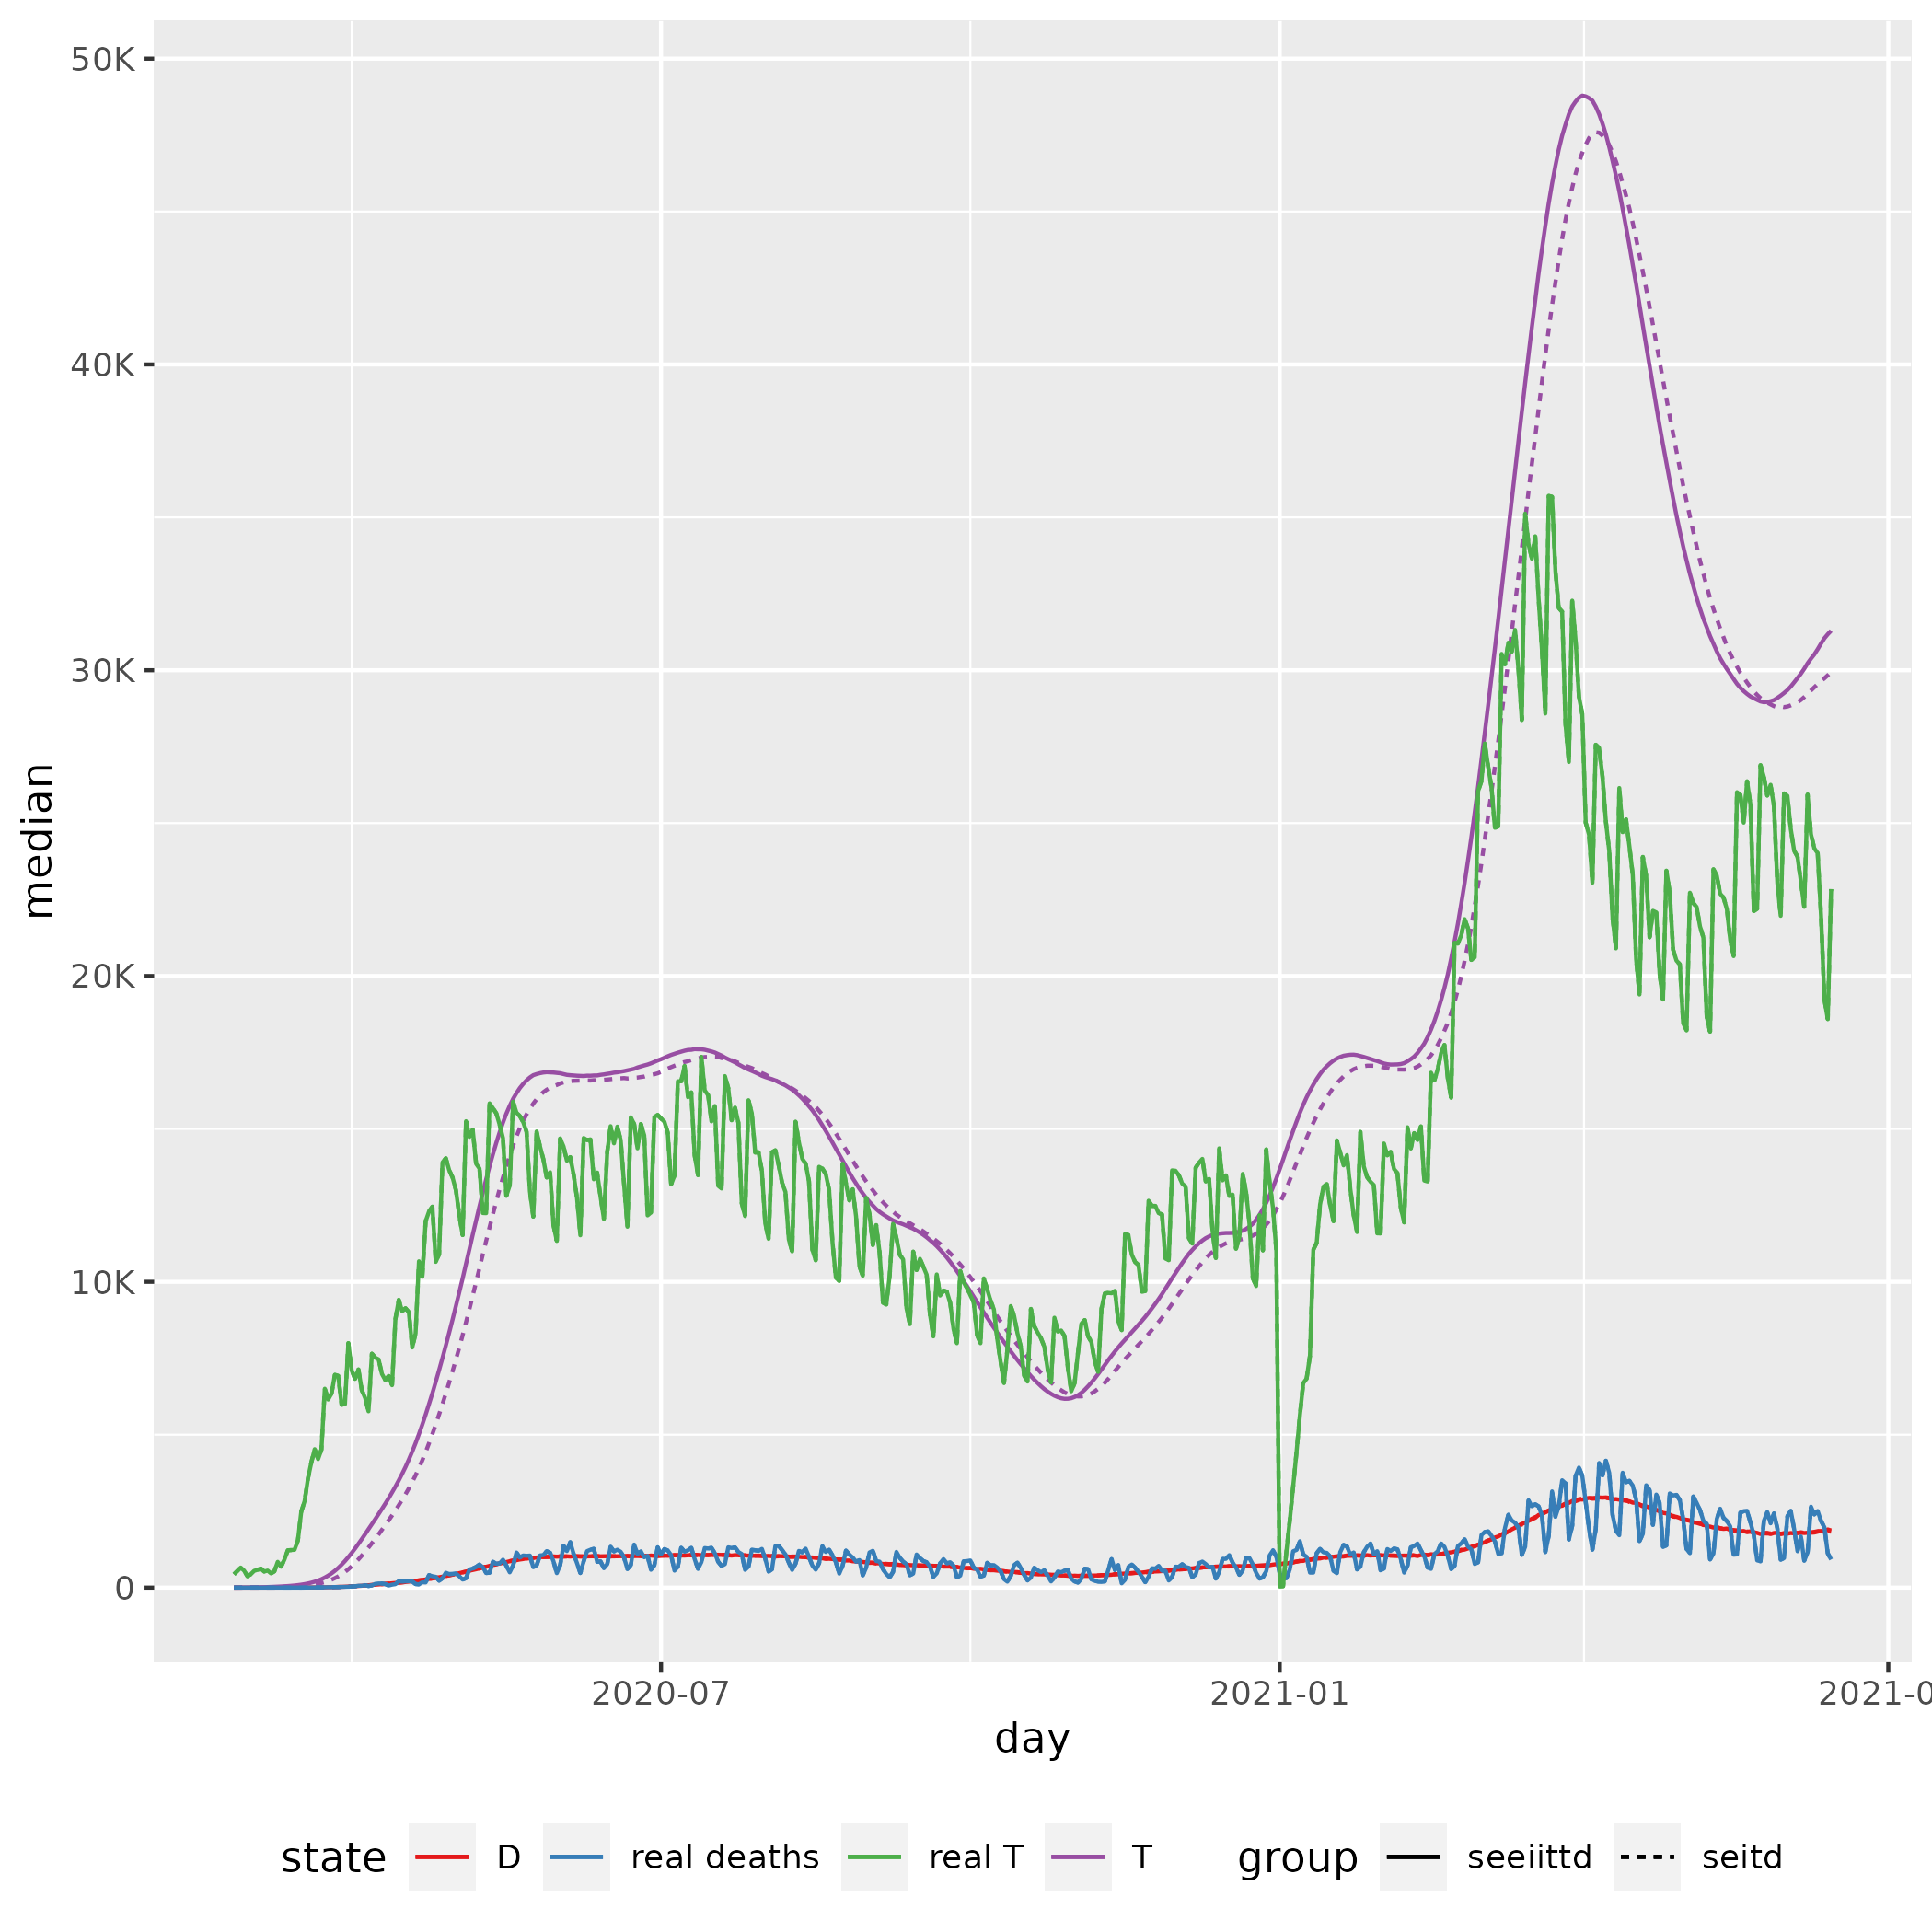
\includegraphics[width=0.45\textwidth]{T_D_seitd_vs_seeiittd_matrix_exp.png}
		\caption{Estimativas do Modelo versus Dados Reais}
		\label{fig:ambidex_performance}
	\end{figure}
\end{frame}

\begin{frame}[allowframebreaks]{Referências}
	\printbibliography
\end{frame}

